% Chapter 4

\chapter{Preparing Dataset} % Main chapter title

\label{Chapter4} % For referencing the chapter elsewhere, use \ref{Chapter4} 

\lhead{Chapter 4. \emph{Preparing Dataset}} % This is for the header on each page - perhaps a shortened title




\section{Introduction}

The data preparation process began with the definition of clear selection criteria. Our objective was to compile recitations from world-class experts to serve as reference models for evaluating Quranic learners. This study focuses exclusively on the Hafs Way (\arb{رواية حفص}) due to its status as the most prevalent recitation method globally.

Acknowledging that manual annotation is prohibitively time-consuming, we developed a data collection pipeline that is approximately 98\% automated. The procedure consists of the following steps:

\begin{enumerate}
\item Selection of a digitized Quranic script as the foundational text.
\item Definition of precise criteria for the \arb{حفص} methodology.
\item Collection of expert recitations.
\item Segmentation of audio at pause points (\arb{وقف}).
\item Transcription of the segmented audio.
\item Data validation using a Tasmeea (\arb{تسميع}) algorithm.
\item Extraction of a phonetic script using our custom Quran Phonetic Script.
\end{enumerate}

For the purposes of this work, a moshaf (\arb{مصحف}) is defined as a complete recitation of the Quran (chapters 1-114) by a single reciter. The statistics of the collected dataset are summarized in Table \ref{tab:all_data_stat}.

\begin{longtable}{|c|c|c|}
\caption{Summary of the proposed dataset. The final collection comprises approximately 848 hours of audio, totaling over 286,000 individual recitation segments.}
\label{tab:all_data_stat}\\
\hline
\textbf{Moshaf ID} & \textbf{Hours} & \textbf{Recitation Count} \\ 
\hline
\endfirsthead
\hline
0.0 & 28.48 & 9,133 \\
\hline
0.1 & 40.31 & 10,764 \\
\hline
0.2 & 49.47 & 9,971 \\
\hline
0.3 & 37.19 & 12,604 \\
\hline
1.0 & 28.41 & 10,939 \\
\hline
2.0 & 51.05 & 9,942 \\
\hline
2.1 & 30.03 & 10,394 \\
\hline
3.0 & 25.19 & 10,444 \\
\hline
4.0 & 29.12 & 10,994 \\
\hline
5.0 & 28.02 & 11,482 \\
\hline
6.0 & 39.39 & 12,435 \\
\hline
7.0 & 28.26 & 9,907 \\
\hline
8.0 & 30.86 & 10,330 \\
\hline
9.0 & 27.95 & 10,642 \\
\hline
11.0 & 24.01 & 10,363 \\
\hline
12.0 & 33.42 & 9,880 \\
\hline
13.0 & 33.99 & 9,377 \\
\hline
19.0 & 30.11 & 11,278 \\
\hline
22.0 & 28.11 & 10,332 \\
\hline
24.0 & 28.51 & 9,868 \\
\hline
25.0 & 16.93 & 7,922 \\
\hline
26.0 & 30.44 & 11,565 \\
\hline
26.1 & 32.71 & 11,850 \\
\hline
27.0 & 28.05 & 11,213 \\
\hline
28.0 & 31.05 & 10,535 \\
\hline
29.0 & 27.79 & 11,061 \\
\hline
30.0 & 29.14 & 11,312 \\
\hline
\textbf{Total} & \textbf{847.99} & \textbf{286,537} \\
\hline
\end{longtable}




% ----------------------------------------------------------------------------------------------------

\section{Choose a Digitized Version of the Holy Quran}

The Quran has multiple digitized versions including Tanzil\footnote{https://tanzil.net} and King Fahd Complex\footnote{https://qurancomplex.gov.sa}. We chose Tanzil because:
\begin{itemize}
\item It uses standard Unicode characters
\item Contains both \arb{إملائي} and \arb{عثماني} versions
\item Maintains high accuracy
\end{itemize}

We excluded KFGQPC due to its evolving/unstable nature compared to Tanzil.



% --------------------------------------------------------------------------------------------------------
\section{Defining Variant Criteria for Hafs}

The Hafs way(\arb{رواية  حفص}) contains several phonetic and prosodic variants. For instance, the application of \arb{مد المنفصل} (Madd Al-Munfasil) can vary in duration, extending for 2, 4, 5, or 6 vowel beats depending on the specific recitational rule. These variants were rigorously defined through an analysis of classical Qira'at literature \cite{al-dabbaa}. The criteria for each variant are summarized in the table below.

To capture this variability, each Moshaf in our dataset is accompanied by a `MoshafAttributes` card that documents its specific recitational features. These cards were manually annotated through a dedicated and meticulous effort, ensuring an accurate representation of each reciter's adherence to the defined rules.



 \subsection{Moshaf Attribute Definitions}
\label{sec:moshaf_attributes}
\begin{itemize}
\item \textbf{rewaya} (\arb{الرواية})
  \begin{itemize}
  \item Values: - \texttt{hafs} (\arb{حفص})
  \item Default Value: 
  \item More Info: The type of the quran Rewaya.
  \end{itemize}

\item \textbf{recitation\_speed} (\arb{سرعة التلاوة})
  \begin{itemize}
  \item Values: 
    \begin{itemize}
    \item  \texttt{mujawad} (\arb{مجود})
    \item  \texttt{above\_murattal} (\arb{فويق المرتل})
    \item  \texttt{murattal} (\arb{مرتل})
    \item  \texttt{hadr} (\arb{حدر})
    \end{itemize}
  \item Default Value: \texttt{murattal} (\arb{مرتل})
  \item More Info: The recitation speed sorted from slowest to the fastest \arb{سرعة التلاوة مرتبة من الأبطأ إلي الأسرع}
  \end{itemize}

\item \textbf{takbeer} (\arb{التكبير})
  \begin{itemize}
  \item Values: 
    \begin{itemize}
    \item  \texttt{no\_takbeer} (\arb{لا تكبير})
    \item  \texttt{beginning\_of\_sharh} (\arb{التكبير من أول الشرح لأول الناس})
    \item  \texttt{end\_of\_doha} (\arb{التكبير من آخر الضحى لآخر الناس})
    \item  \texttt{general\_takbeer} (\arb{التكبير أول كل سورة إلا التوبة})
    \end{itemize}
  \item Default Value: \texttt{no\_takbeer} (\arb{لا تكبير})
  \item More Info: The ways to add takbeer (\arb{الله أكبر}) after Istiaatha (\arb{استعاذة}) and between end of the surah and beginning of the surah. \texttt{no\_takbeer}: "\arb{لا تكبير}" — No Takbeer (No proclamation of greatness, i.e., there is no Takbeer recitation) \texttt{beginning\_of\_sharh}: "\arb{التكبير من أول الشرح لأول الناس}" — Takbeer from the beginning of Surah Ash-Sharh to the beginning of Surah An-Nas \texttt{end\_of\_dohaf}: "\arb{التكبير من آخر الضحى لآخر الناس}" — Takbeer from the end of Surah Ad-Duha to the end of Surah An-Nas \texttt{general\_takbeer}: "\arb{التكبير أول كل سورة إلا التوبة}" — Takbeer at the beginning of every Surah except Surah At-Tawbah
  \end{itemize}

\item \textbf{madd\_monfasel\_len} (\arb{مد المنفصل})
  \begin{itemize}
  \item Values: 
    \begin{itemize}
    \item  \texttt{2}
    \item  \texttt{3}
    \item  \texttt{4}
    \item  \texttt{5}
    \end{itemize}
  \item Default Value: 
  \item More Info: The length of Mad Al Monfasel "\arb{مد المنفصل}" for Hafs Rewaya.
  \end{itemize}

\item \textbf{madd\_mottasel\_len} (\arb{مقدار المد المتصل})
  \begin{itemize}
  \item Values: 
    \begin{itemize}
    \item  \texttt{4}
    \item  \texttt{5}
    \item  \texttt{6}
    \end{itemize}
  \item Default Value: 
  \item More Info: The length of Mad Al Motasel "\arb{مد المتصل}" for Hafs.
  \end{itemize}

\item \textbf{madd\_mottasel\_waqf} (\arb{مقدار المد المتصل وقفا})
  \begin{itemize}
  \item Values: 
    \begin{itemize}
    \item  \texttt{4}
    \item  \texttt{5}
    \item  \texttt{6}
    \end{itemize}
  \item Default Value: 
  \item More Info: The length of Madd Almotasel at pause for Hafs.. Example "\arb{السماء}".
  \end{itemize}

\item \textbf{madd\_aared\_len} (\arb{مقدار المد العارض})
  \begin{itemize}
  \item Values: 
    \begin{itemize}
    \item  \texttt{2}
    \item  \texttt{4}
    \item  \texttt{6}
    \end{itemize}
  \item Default Value: 
  \item More Info: The length of Mad Al Aared "\arb{مد العارض للسكون}".
  \end{itemize}

\item \textbf{madd\_alleen\_len} (\arb{مقدار مد اللين})
  \begin{itemize}
  \item Values: 
    \begin{itemize}
    \item  \texttt{2}
    \item  \texttt{4}
    \item  \texttt{6}
    \end{itemize}
  \item Default Value: \texttt{None}
  \item More Info: The length of the Madd al-Leen when stopping at the end of a word (for a sakin waw or ya preceded by a letter with a fatha) should be less than or equal to the length of Madd al-'Arid (the temporary stretch due to stopping). \textbf{Default Value is equal to \texttt{madd\_aared\_len}}. \arb{مقدار مد اللين عن القوف (للواو الساكنة والياء الساكنة وقبلها حرف مفتوح) ويجب أن يكون مقدار مد اللين أقل من أو يساوي مع العارض}
  \end{itemize}

\item \textbf{ghonna\_lam\_and\_raa} (\arb{غنة اللام و الراء})
  \begin{itemize}
  \item Values: 
    \begin{itemize}
    \item  \texttt{ghonna} (\arb{غنة})
    \item  \texttt{no\_ghonna} (\arb{لا غنة})
    \end{itemize}
  \item Default Value: \texttt{no\_ghonna} (\arb{لا غنة})
  \item More Info: The ghonna for merging (Idghaam) noon with Lam and Raa for Hafs.
  \end{itemize}

\item \textbf{meem\_aal\_imran} (\arb{ميم آل عمران في قوله تعالى: \{الم الله\} وصلا})
  \begin{itemize}
  \item Values: 
    \begin{itemize}
    \item  \texttt{waqf} (\arb{وقف})
    \item  \texttt{wasl\_2} (\arb{فتح الميم ومدها حركتين})
    \item  \texttt{wasl\_6} (\arb{فتح الميم ومدها ستة حركات})
    \end{itemize}
  \item Default Value: \texttt{waqf} (\arb{وقف})
  \item More Info: The ways to recite the word meem Aal Imran (\arb{الم الله}) at connected recitation. \texttt{waqf}: Pause with a prolonged madd (elongation) of 6 harakat (beats). \texttt{wasl\_2} Pronounce "meem" with fathah (a short "a" sound) and stretch it for 2 harakat. \texttt{wasl\_6} Pronounce "meem" with fathah and stretch it for 6 harakat.
  \end{itemize}

\item \textbf{madd\_yaa\_alayn\_alharfy} (\arb{مقدار   المد اللازم الحرفي للعين})
  \begin{itemize}
  \item Values: 
    \begin{itemize}
    \item  \texttt{2}
    \item  \texttt{4}
    \item  \texttt{6}
    \end{itemize}
  \item Default Value: \texttt{6}
  \item More Info: The length of Lzem Harfy of Yaa in letter Al-Ayen Madd "\arb{المد الحرفي اللازم لحرف العين}" in surar: Maryam "\arb{مريم}", AlShura "\arb{الشورى}".
  \end{itemize}

\item \textbf{saken\_before\_hamz} (\arb{الساكن قبل الهمز})
  \begin{itemize}
  \item Values: 
    \begin{itemize}
    \item  \texttt{tahqeek} (\arb{تحقيق})
    \item  \texttt{general\_sakt} (\arb{سكت عام})
    \item  \texttt{local\_sakt} (\arb{سكت خاص})
    \end{itemize}
  \item Default Value: \texttt{tahqeek} (\arb{تحقيق})
  \item More Info: The ways of Hafs for saken before hamz. "The letter with sukoon before the hamzah (\arb{ء})".And it has three forms: full articulation (\texttt{tahqeeq}), general pause (\texttt{general\_sakt}), and specific pause (\texttt{local\_skat}).
  \end{itemize}

\item \textbf{sakt\_iwaja} (\arb{السكت عند عوجا في الكهف})
  \begin{itemize}
  \item Values: 
    \begin{itemize}
    \item  \texttt{sakt} (\arb{سكت})
    \item  \texttt{waqf} (\arb{وقف})
    \item  \texttt{idraj} (\arb{إدراج})
    \end{itemize}
  \item Default Value: \texttt{waqf} (\arb{وقف})
  \item More Info: The ways to recite the word "\arb{عوجا}" (Iwaja). \texttt{sakt} means slight pause. \texttt{idraj} means not \texttt{sakt}. \texttt{waqf}: means full pause, so we can not determine whether the reciter uses \texttt{sakt} or \texttt{idraj} (no sakt).
  \end{itemize}

\item \textbf{sakt\_marqdena} (\arb{السكت عند مرقدنا  في يس})
  \begin{itemize}
  \item Values: 
    \begin{itemize}
    \item  \texttt{sakt} (\arb{سكت})
    \item  \texttt{waqf} (\arb{وقف})
    \item  \texttt{idraj} (\arb{إدراج})
    \end{itemize}
  \item Default Value: \texttt{waqf} (\arb{وقف})
  \item More Info: The ways to recite the word "\arb{مرقدنا}" (Marqadena) in Surat Yassen. \texttt{sakt} means slight pause. \texttt{idraj} means not \texttt{sakt}. \texttt{waqf}: means full pause, so we can not determine whether the reciter uses \texttt{sakt} or \texttt{idraj} (no sakt).
  \end{itemize}

\item \textbf{sakt\_man\_raq} (\arb{السكت عند  من راق في القيامة})
  \begin{itemize}
  \item Values: 
    \begin{itemize}
    \item  \texttt{sakt} (\arb{سكت})
    \item  \texttt{waqf} (\arb{وقف})
    \item  \texttt{idraj} (\arb{إدراج})
    \end{itemize}
  \item Default Value: \texttt{sakt} (\arb{سكت})
  \item More Info: The ways to recite the word "\arb{من راق}" (Man Raq) in Surat Al Qiyama. \texttt{sakt} means slight pause. \texttt{idraj} means not \texttt{sakt}. \texttt{waqf}: means full pause, so we can not determine whether the reciter uses \texttt{sakt} or \texttt{idraj} (no sakt).
  \end{itemize}

\item \textbf{sakt\_bal\_ran} (\arb{السكت عند  بل ران في  المطففين})
  \begin{itemize}
  \item Values: 
    \begin{itemize}
    \item  \texttt{sakt} (\arb{سكت})
    \item  \texttt{waqf} (\arb{وقف})
    \item  \texttt{idraj} (\arb{إدراج})
    \end{itemize}
  \item Default Value: \texttt{sakt} (\arb{سكت})
  \item More Info: The ways to recite the word "\arb{بل ران}" (Bal Ran) in Surat Al Motaffin. \texttt{sakt} means slight pause. \texttt{idraj} means not \texttt{sakt}. \texttt{waqf}: means full pause, so we can not determine whether the reciter uses \texttt{sakt} or \texttt{idraj} (no sakt).
  \end{itemize}

\item \textbf{sakt\_maleeyah} (\arb{وجه  قوله تعالى \{ماليه هلك\} بالحاقة})
  \begin{itemize}
  \item Values: 
    \begin{itemize}
    \item  \texttt{sakt} (\arb{سكت})
    \item  \texttt{waqf} (\arb{وقف})
    \item  \texttt{idgham} (\arb{إدغام})
    \end{itemize}
  \item Default Value: \texttt{waqf} (\arb{وقف})
  \item More Info: The ways to recite the word \{\arb{ماليه هلك}\} in Surah Al-Ahqaf. \texttt{sakt} means slight pause. \texttt{idgham} Assimilation of the letter 'Ha' (\arb{ه}) into the letter 'Ha' (\arb{ه}) with complete assimilation.\texttt{waqf}: means full pause, so we can not determine whether the reciter uses \texttt{sakt} or \texttt{idgham}.
  \end{itemize}

\item \textbf{between\_anfal\_and\_tawba} (\arb{وجه بين الأنفال والتوبة})
  \begin{itemize}
  \item Values: 
    \begin{itemize}
    \item  \texttt{waqf} (\arb{وقف})
    \item  \texttt{sakt} (\arb{سكت})
    \item  \texttt{wasl} (\arb{وصل})
    \end{itemize}
  \item Default Value: \texttt{waqf} (\arb{وقف})
  \item More Info: The ways to recite end of Surah Al-Anfal and beginning of Surah At-Tawbah.
  \end{itemize}

\item \textbf{noon\_and\_yaseen} (\arb{الإدغام والإظهار في النون عند الواو من قوله تعالى: \{يس والقرآن\}و \{ن والقلم\}})
  \begin{itemize}
  \item Values: 
    \begin{itemize}
    \item  \texttt{izhar} (\arb{إظهار})
    \item  \texttt{idgham} (\arb{إدغام})
    \end{itemize}
  \item Default Value: \texttt{izhar} (\arb{إظهار})
  \item More Info: Whether to merge noon of both: \{\arb{يس}\} and \{\arb{ن}\} with (\arb{و}) "\texttt{idgham}" or not "\texttt{izhar}".
  \end{itemize}

\item \textbf{yaa\_ataan} (\arb{إثبات الياء وحذفها وقفا في قوله تعالى \{آتان\} بالنمل})
  \begin{itemize}
  \item Values: 
    \begin{itemize}
    \item  \texttt{wasl} (\arb{وصل})
    \item  \texttt{hadhf} (\arb{حذف})
    \item  \texttt{ithbat} (\arb{إثبات})
    \end{itemize}
  \item Default Value: \texttt{wasl} (\arb{وصل})
  \item More Info: The affirmation and omission of the letter 'Yaa' in the pause of the verse \{\arb{آتاني}\} in Surah An-Naml. \texttt{wasl}: means connected recitation without pausing as (\arb{آتانيَ}). \texttt{hadhf}: means deletion of letter (\arb{ي}) at pause so recited as (\arb{آتان}). \texttt{ithbat}: means confirmation reciting letter (\arb{ي}) at pause as (\arb{آتاني}).
  \end{itemize}

\item \textbf{start\_with\_ism} (\arb{وجه البدأ بكلمة \{الاسم\} في سورة الحجرات})
  \begin{itemize}
  \item Values: 
    \begin{itemize}
    \item  \texttt{wasl} (\arb{وصل})
    \item  \texttt{lism} (\arb{لسم})
    \item  \texttt{alism} (\arb{ألسم})
    \end{itemize}
  \item Default Value: \texttt{wasl} (\arb{وصل})
  \item More Info: The ruling on starting with the word \{\arb{الاسم}\} in Surah Al-Hujurat. \texttt{lism} Recited as (\arb{لسم}) at the beginning. \texttt{alism} Recited as (\arb{ألسم}). \texttt{wasl}: means completing recitation without pausing as normal, So Reciting is as (\arb{بئس لسم}).
  \end{itemize}

\item \textbf{yabsut} (\arb{السين والصاد في قوله تعالى: \{والله يقبض ويبسط\} بالبقرة})
  \begin{itemize}
  \item Values: 
    \begin{itemize}
    \item  \texttt{seen} (\arb{سين})
    \item  \texttt{saad} (\arb{صاد})
    \end{itemize}
  \item Default Value: \texttt{seen} (\arb{سين})
  \item More Info: The ruling on pronouncing \texttt{seen} (\arb{س}) or \texttt{saad} (\arb{ص}) in the verse \{\arb{والله يقبض ويبسط}\} in Surah Al-Baqarah.
  \end{itemize}

\item \textbf{bastah} (\arb{السين والصاد في قوله تعالى:  \{وزادكم في الخلق بسطة\} بالأعراف})
  \begin{itemize}
  \item Values: 
    \begin{itemize}
    \item  \texttt{seen} (\arb{سين})
    \item  \texttt{saad} (\arb{صاد})
    \end{itemize}
  \item Default Value: \texttt{seen} (\arb{سين})
  \item More Info: The ruling on pronouncing \texttt{seen} (\arb{س}) or \texttt{saad} (\arb{ص}) in the verse \{\arb{وزادكم في الخلق بسطة}\} in Surah Al-A'raf.
  \end{itemize}

\item \textbf{almusaytirun} (\arb{السين والصاد في قوله تعالى \{أم هم المصيطرون\} بالطور})
  \begin{itemize}
  \item Values: 
    \begin{itemize}
    \item  \texttt{seen} (\arb{سين})
    \item  \texttt{saad} (\arb{صاد})
    \end{itemize}
  \item Default Value: \texttt{saad} (\arb{صاد})
  \item More Info: The pronunciation of \texttt{seen} (\arb{س}) or \texttt{saad} (\arb{ص}) in the verse \{\arb{أم هم المصيطرون}\} in Surah At-Tur.
  \end{itemize}

\item \textbf{bimusaytir} (\arb{السين والصاد في قوله تعالى:  \{لست عليهم بمصيطر\} بالغاشية})
  \begin{itemize}
  \item Values: 
    \begin{itemize}
    \item  \texttt{seen} (\arb{سين})
    \item  \texttt{saad} (\arb{صاد})
    \end{itemize}
  \item Default Value: \texttt{saad} (\arb{صاد})
  \item More Info: The pronunciation of \texttt{seen} (\arb{س}) or \texttt{saad} (\arb{ص}) in the verse \{\arb{لست عليهم بمصيطر}\} in Surah Al-Ghashiyah.
  \end{itemize}

\item \textbf{tasheel\_or\_madd} (\arb{همزة الوصل في قوله تعالى: \{آلذكرين\} بموضعي الأنعام و\{آلآن\} موضعي يونس و\{آلله\} بيونس والنمل})
  \begin{itemize}
  \item Values: 
    \begin{itemize}
    \item  \texttt{tasheel} (\arb{تسهيل})
    \item  \texttt{madd} (\arb{مد})
    \end{itemize}
  \item Default Value: \texttt{madd} (\arb{مد})
  \item More Info: Tasheel of Madd "\arb{وجع التسهيل أو المد}" for 6 words in The Holy Quran: "\arb{ءالذكرين}", "\arb{ءالله}", "\arb{ءائن}".
  \end{itemize}

\item \textbf{yalhath\_dhalik} (\arb{الإدغام وعدمه في قوله تعالى: \{يلهث ذلك\} بالأعراف})
  \begin{itemize}
  \item Values: 
    \begin{itemize}
    \item  \texttt{izhar} (\arb{إظهار})
    \item  \texttt{idgham} (\arb{إدغام})
    \item  \texttt{waqf} (\arb{وقف})
    \end{itemize}
  \item Default Value: \texttt{idgham} (\arb{إدغام})
  \item More Info: The assimilation (\texttt{idgham}) and non-assimilation (\texttt{izhar}) in the verse \{\arb{يلهث ذلك}\} in Surah Al-A'raf. \texttt{waqf}: means the reciter has paused on (\arb{يلهث})
  \end{itemize}

\item \textbf{irkab\_maana} (\arb{الإدغام والإظهار في قوله تعالى: \{اركب معنا\} بهود})
  \begin{itemize}
  \item Values: 
    \begin{itemize}
    \item  \texttt{izhar} (\arb{إظهار})
    \item  \texttt{idgham} (\arb{إدغام})
    \item  \texttt{waqf} (\arb{وقف})
    \end{itemize}
  \item Default Value: \texttt{idgham} (\arb{إدغام})
  \item More Info: The assimilation and clear pronunciation in the verse \{\arb{اركب معنا}\} in Surah Hud. This refers to the recitation rules concerning whether the letter "Noon" (\arb{ن}) is assimilated into the following letter or pronounced clearly when reciting this specific verse. \texttt{waqf}: means the reciter has paused on (\arb{اركب})
  \end{itemize}

\item \textbf{noon\_tamnna} (\arb{الإشمام والروم (الاختلاس) في قوله تعالى \{لا تأمنا على يوسف\}})
  \begin{itemize}
  \item Values: 
    \begin{itemize}
    \item  \texttt{ishmam} (\arb{إشمام})
    \item  \texttt{rawm} (\arb{روم})
    \end{itemize}
  \item Default Value: \texttt{ishmam} (\arb{إشمام})
  \item More Info: The nasalization (\texttt{ishmam}) or the slight drawing (\texttt{rawm}) in the verse \{\arb{لا تأمنا على يوسف}\}
  \end{itemize}

\item \textbf{harakat\_daaf} (\arb{حركة الضاد (فتح أو ضم) في قوله تعالى \{ضعف\} بالروم})
  \begin{itemize}
  \item Values: 
    \begin{itemize}
    \item  \texttt{fath} (\arb{فتح})
    \item  \texttt{dam} (\arb{ضم})
    \end{itemize}
  \item Default Value: \texttt{fath} (\arb{فتح})
  \item More Info: The vowel movement of the letter 'Dhad' (\arb{ض}) (whether with \texttt{fath} or \texttt{dam}) in the word \{\arb{ضعف}\} in Surah Ar-Rum.
  \end{itemize}

\item \textbf{alif\_salasila} (\arb{إثبات الألف وحذفها وقفا في قوله تعالى: \{سلاسلا\} بسورة الإنسان})
  \begin{itemize}
  \item Values: 
    \begin{itemize}
    \item  \texttt{hadhf} (\arb{حذف})
    \item  \texttt{ithbat} (\arb{إثبات})
    \item  \texttt{wasl} (\arb{وصل})
    \end{itemize}
  \item Default Value: \texttt{wasl} (\arb{وصل})
  \item More Info: Affirmation and omission of the 'Alif' when pausing in the verse \{\arb{سلاسلا}\} in Surah Al-Insan. This refers to the recitation rule regarding whether the final "Alif" in the word "\arb{سلاسلا}" is pronounced (affirmed) or omitted when pausing (waqf) at this word during recitation in the specific verse from Surah Al-Insan. \texttt{hadhf}: means to remove alif (\arb{ا}) during pause as (\arb{سلاسل}) \texttt{ithbat}: means to recite alif (\arb{ا}) during pause as (\arb{سلاسلا}) \texttt{wasl} means completing the recitation as normal without pausing, so recite it as (\arb{سلاسلَ وأغلالا})
  \end{itemize}

\item \textbf{idgham\_nakhluqkum} (\arb{إدغام القاف في الكاف إدغاما ناقصا أو كاملا \{نخلقكم\} بالمرسلات})
  \begin{itemize}
  \item Values: 
    \begin{itemize}
    \item  \texttt{idgham\_kamil} (\arb{إدغام كامل})
    \item  \texttt{idgham\_naqis} (\arb{إدغام ناقص})
    \end{itemize}
  \item Default Value: \texttt{idgham\_kamil} (\arb{إدغام كامل})
  \item More Info: Assimilation of the letter 'Qaf' into the letter 'Kaf,' whether incomplete (\texttt{idgham\_naqis}) or complete (\texttt{idgham\_kamil}), in the verse \{\arb{نخلقكم}\} in Surah Al-Mursalat.
  \end{itemize}

\item \textbf{raa\_firq} (\arb{التفخيم والترقيق في راء \{فرق\} في الشعراء وصلا})
  \begin{itemize}
  \item Values: 
    \begin{itemize}
    \item  \texttt{waqf} (\arb{وقف})
    \item  \texttt{tafkheem} (\arb{تفخيم})
    \item  \texttt{tarqeeq} (\arb{ترقيق})
    \end{itemize}
  \item Default Value: \texttt{tafkheem} (\arb{تفخيم})
  \item More Info: Emphasis and softening of the letter 'Ra' in the word \{\arb{فرق}\} in Surah Ash-Shu'ara' when connected (wasl). This refers to the recitation rules concerning whether the letter "Ra" (\arb{ر}) in the word "\arb{فرق}" is pronounced with emphasis (\texttt{tafkheem}) or softening (\texttt{tarqeeq}) when reciting the specific verse from Surah Ash-Shu'ara' in connected speech. \texttt{waqf}: means pausing so we only have one way (tafkheem of Raa)
  \end{itemize}

\item \textbf{raa\_alqitr} (\arb{التفخيم والترقيق في راء \{القطر\} في سبأ وقفا})
  \begin{itemize}
  \item Values: 
    \begin{itemize}
    \item  \texttt{wasl} (\arb{وصل})
    \item  \texttt{tafkheem} (\arb{تفخيم})
    \item  \texttt{tarqeeq} (\arb{ترقيق})
    \end{itemize}
  \item Default Value: \texttt{wasl} (\arb{وصل})
  \item More Info: Emphasis and softening of the letter 'Ra' in the word \{\arb{القطر}\} in Surah Saba' when pausing (waqf). This refers to the recitation rules regarding whether the letter "Ra" (\arb{ر}) in the word "\arb{القطر}" is pronounced with emphasis (\texttt{tafkheem}) or softening (\texttt{tarqeeq}) when pausing at this word in Surah Saba'. \texttt{wasl}: means not pausing so we only have one way (tarqeeq of Raa)
  \end{itemize}

\item \textbf{raa\_misr} (\arb{التفخيم والترقيق في راء \{مصر\} في يونس وموضعي يوسف والزخرف  وقفا})
  \begin{itemize}
  \item Values: 
    \begin{itemize}
    \item  \texttt{wasl} (\arb{وصل})
    \item  \texttt{tafkheem} (\arb{تفخيم})
    \item  \texttt{tarqeeq} (\arb{ترقيق})
    \end{itemize}
  \item Default Value: \texttt{wasl} (\arb{وصل})
  \item More Info: Emphasis and softening of the letter 'Ra' in the word \{\arb{مصر}\} in Surah Yunus, and in the locations of Surah Yusuf and Surah Az-Zukhruf when pausing (waqf). This refers to the recitation rules regarding whether the letter "Ra" (\arb{ر}) in the word "\arb{مصر}" is pronounced with emphasis (\texttt{tafkheem}) or softening (\texttt{tarqeeq}) at the specific pauses in these Surahs. \texttt{wasl}: means not pausing so we only have one way (tafkheem of Raa)
  \end{itemize}

\item \textbf{raa\_nudhur} (\arb{التفخيم والترقيق  في راء \{نذر\} بالقمر وقفا})
  \begin{itemize}
  \item Values: 
    \begin{itemize}
    \item  \texttt{wasl} (\arb{وصل})
    \item  \texttt{tafkheem} (\arb{تفخيم})
    \item  \texttt{tarqeeq} (\arb{ترقيق})
    \end{itemize}
  \item Default Value: \texttt{tafkheem} (\arb{تفخيم})
  \item More Info: Emphasis and softening of the letter 'Ra' in the word \{\arb{نذر}\} in Surah Al-Qamar when pausing (waqf). This refers to the recitation rules regarding whether the letter "Ra" (\arb{ر}) in the word "\arb{نذر}" is pronounced with emphasis (\texttt{tafkheem}) or softening (\texttt{tarqeeq}) when pausing at this word in Surah Al-Qamar. \texttt{wasl}: means not pausing so we only have one way (tarqeeq of Raa)
  \end{itemize}

\item \textbf{raa\_yasr} (\arb{التفخيم والترقيق في راء \{يسر\} بالفجر و\{أن أسر\} بطه والشعراء و\{فأسر\} بهود والحجر والدخان  وقفا})
  \begin{itemize}
  \item Values: 
    \begin{itemize}
    \item  \texttt{wasl} (\arb{وصل})
    \item  \texttt{tafkheem} (\arb{تفخيم})
    \item  \texttt{tarqeeq} (\arb{ترقيق})
    \end{itemize}
  \item Default Value: \texttt{tarqeeq} (\arb{ترقيق})
  \item More Info: Emphasis and softening of the letter 'Ra' in the word \{\arb{يسر}\} in Surah Al-Fajr when pausing (waqf). This refers to the recitation rules regarding whether the letter "Ra" (\arb{ر}) in the word "\arb{يسر}" is pronounced with emphasis (\texttt{tafkheem}) or softening (\texttt{tarqeeq}) when pausing at this word in Surah Al-Fajr. \texttt{wasl}: means not pausing so we only have one way (tarqeeq of Raa)
  \end{itemize}

\item \textbf{meem\_mokhfah} (\arb{هل الميم مخفاة أو مدغمة})
  \begin{itemize}
  \item Values: 
    \begin{itemize}
    \item  \texttt{meem} (\arb{ميم})
    \item  \texttt{ikhfaa} (\arb{إخفاء})
    \end{itemize}
  \item Default Value: \texttt{ikhfaa} (\arb{إخفاء})
  \item More Info: This is not a \textbf{standard} Hafs way but a disagreement between \textbf{scholars} in our century on how to \textbf{pronounce} \textbf{Ikhfa} for meem. Some \textbf{scholars} do full merging (\arb{إدغام}) and the others open the \textbf{lips} a little bit (\arb{إخفاء}). We did not want to add this, but some of the best reciters disagree about this.
  \end{itemize}
\end{itemize}


% --------------------------------------------------------------------------

\section{Collection of Expert Recitations}

Recitations were collected from 22 world-class reciters, amounting to a total of \textbf{893 hours} of audio before filtering. The collection process prioritized premium audio quality.

\begin{figure}[H]
\centering
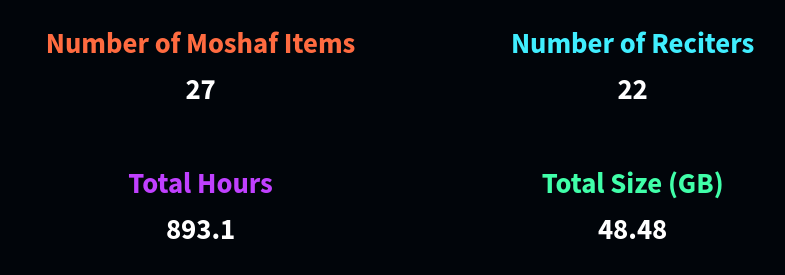
\includegraphics[width=0.8\textwidth]{../figures/stats.png}
\caption{Overview statistics of the collected audio database.}
\label{fig:stats}
\end{figure}

\begin{figure}[H]
\centering
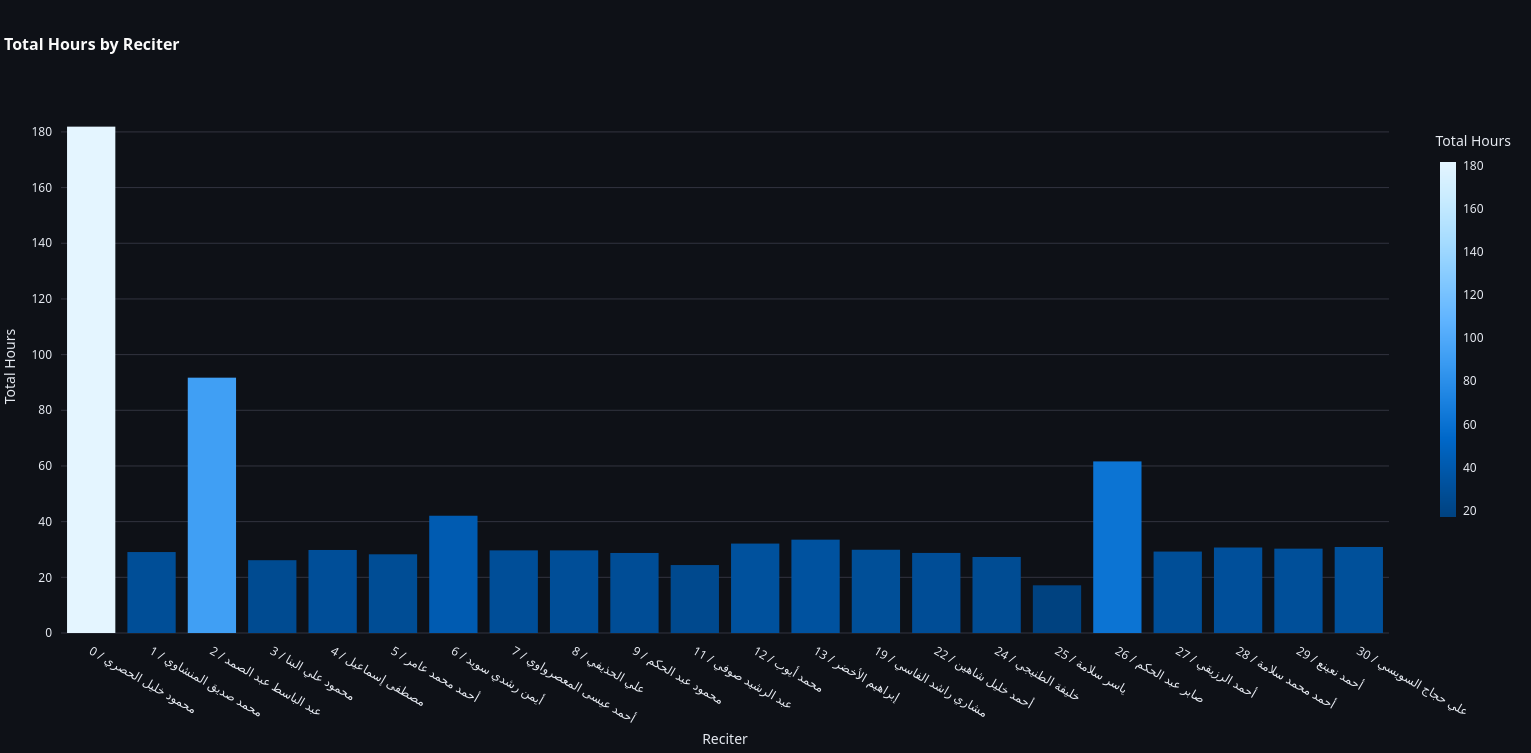
\includegraphics[width=0.8\textwidth]{./figures/reciter.png}
\caption{Total duration of collected recitations, broken down by individual reciter.}
\label{fig:reciter}
\end{figure}

To facilitate this collection, a web GUI was developed using Streamlit\footnote{https://streamlit.io/}. This application performs the following tasks:
\begin{itemize}
\item Downloads audio tracks and extracts their metadata.
\item Organizes the data by Moshaf, with each chapter saved as a separate file (e.g., `001.mp3`).
\item Provides an interface for annotating Moshaf attribute cards.
\end{itemize}

\subsection{Running the Collection Application}

\subsubsection{Cloning the Repository}
The application source code can be obtained by cloning the Git repository:
\begin{lstlisting}[language=bash]
git clone https://github.com/obadx/prepare-quran-dataset
\end{lstlisting}

\subsubsection{Installing `uv`}
The project uses `uv` for dependency management. It can be installed via `pip`:
\begin{lstlisting}[language=bash]
pip install uv
\end{lstlisting}
Alternatively, it can be installed directly from the official installer:
\begin{lstlisting}[language=bash]
curl -LsSf https://astral.sh/uv/install.sh | sh
\end{lstlisting}

\subsubsection{Installing Project Dependencies}
Navigate to the project directory and sync the dependencies, including those for annotation:
\begin{lstlisting}[language=bash]
cd prepare-quran-dataset
uv sync --extra annotate
\end{lstlisting}

\subsubsection{Installing Frontend Dependencies}
The frontend has additional requirements. Navigate to its directory and install them:
\begin{lstlisting}[language=bash]
cd frontend
uv pip install -r requirements.txt
\end{lstlisting}

\subsubsection{Launching the Frontend Application}
With dependencies installed, the Streamlit application can be launched from the `frontend` directory:
\begin{lstlisting}[language=bash]
streamlit run streamlit_app.py
\end{lstlisting}

\subsection{UI Snapshots}

\begin{figure}[H]
\centering
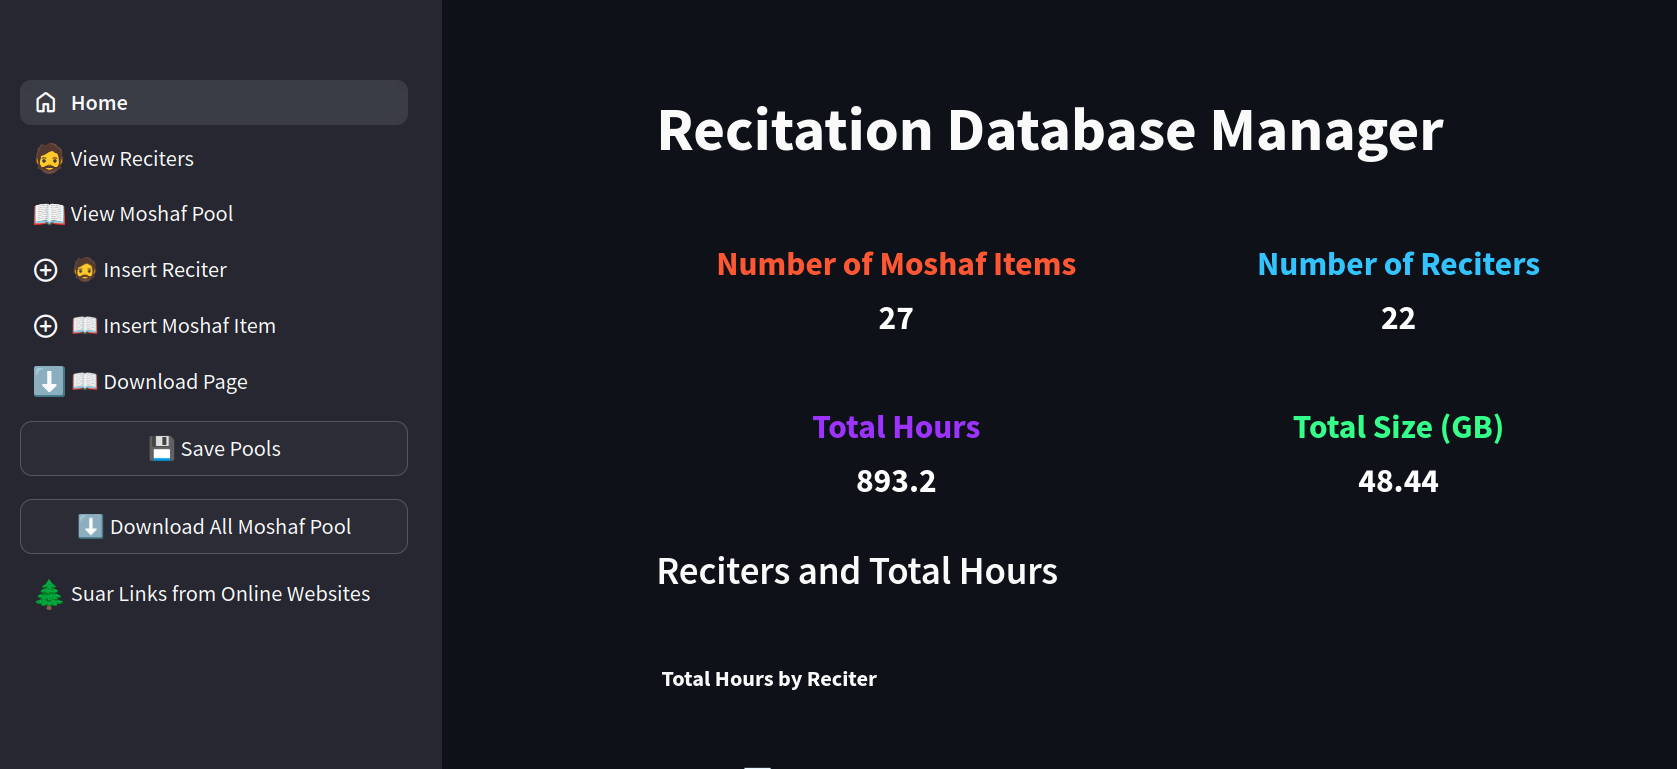
\includegraphics[width=0.8\textwidth]{../figures/ui_main_page.png}
\caption{The main page of the custom annotation platform.}
\label{fig:ui_main}
\end{figure}

\begin{figure}[H]
\centering
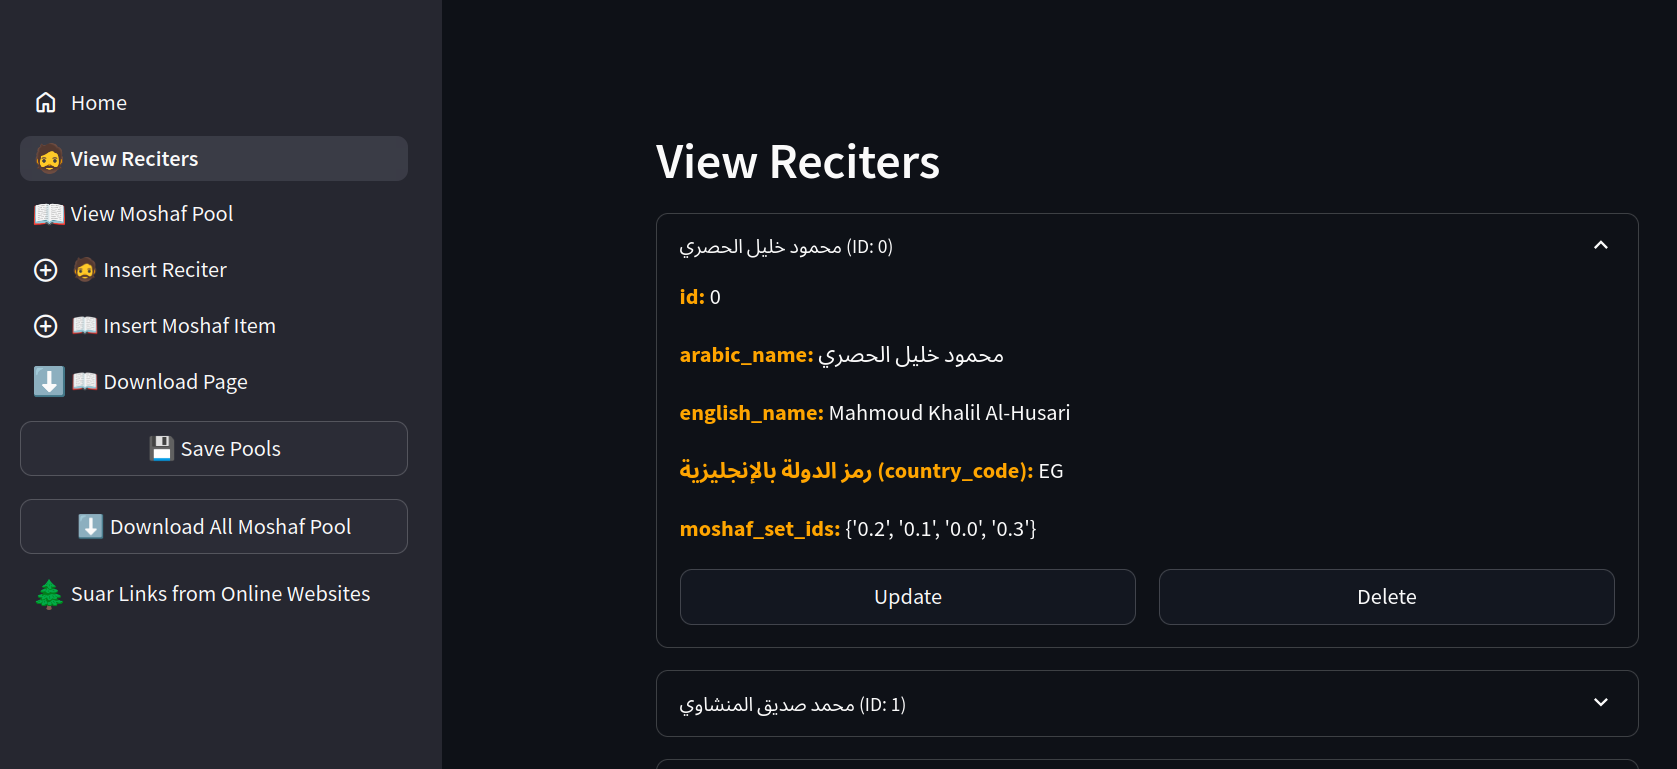
\includegraphics[width=0.8\textwidth]{../figures/ui_veiw_reciters.png}
\caption{The reciter management view within the application.}
\label{fig:ui_reciters}
\end{figure}

\begin{figure}[H]
\centering
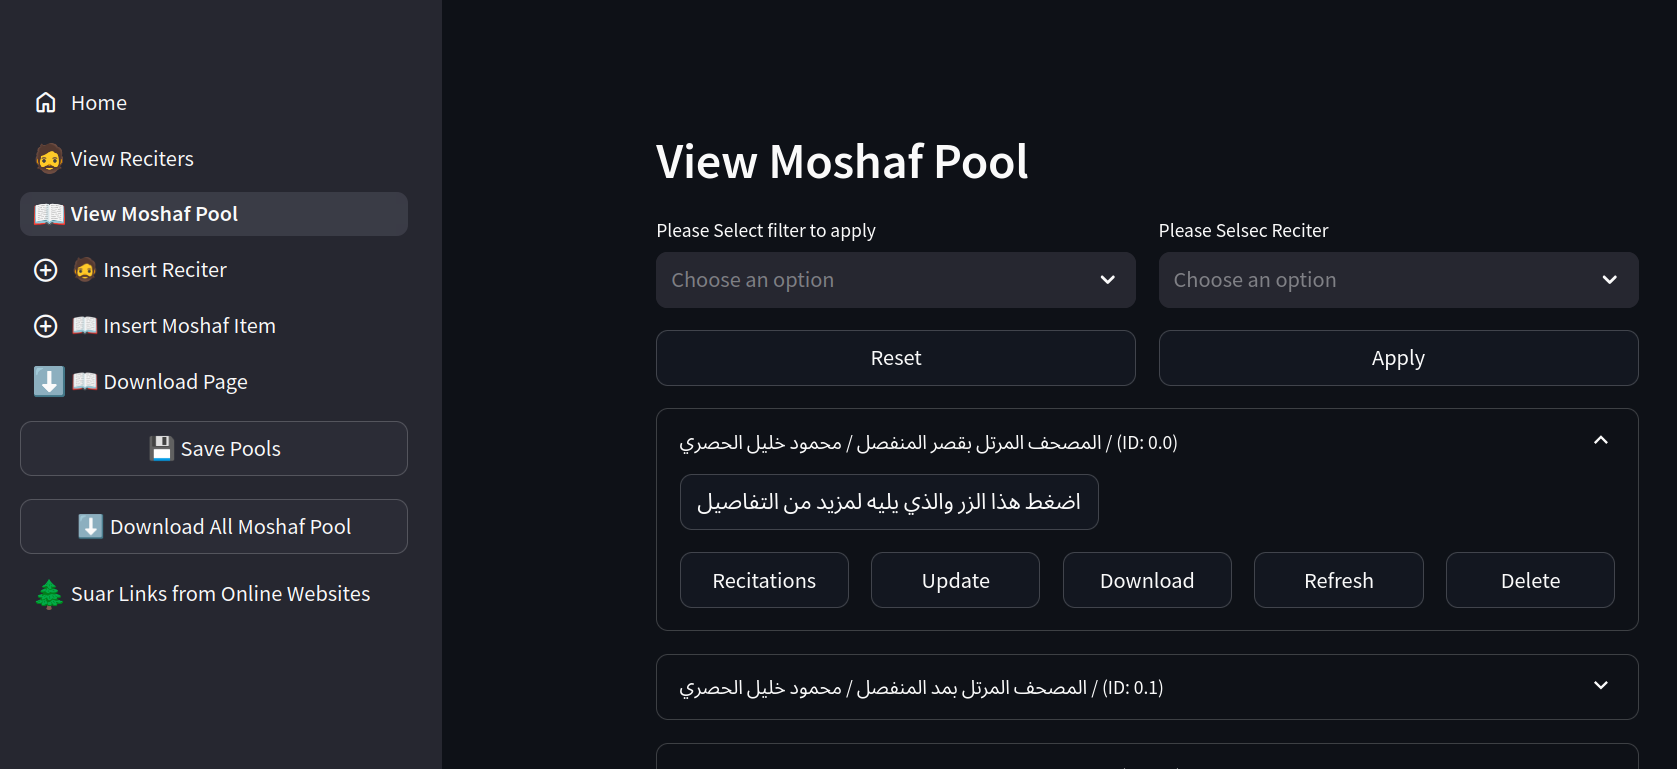
\includegraphics[width=0.8\textwidth]{../figures/ui_veiw_all_moshaf.png}
\caption{View displaying all available Masahif in the database.}
\label{fig:ui_masahif}
\end{figure}

\begin{figure}[H]
\centering
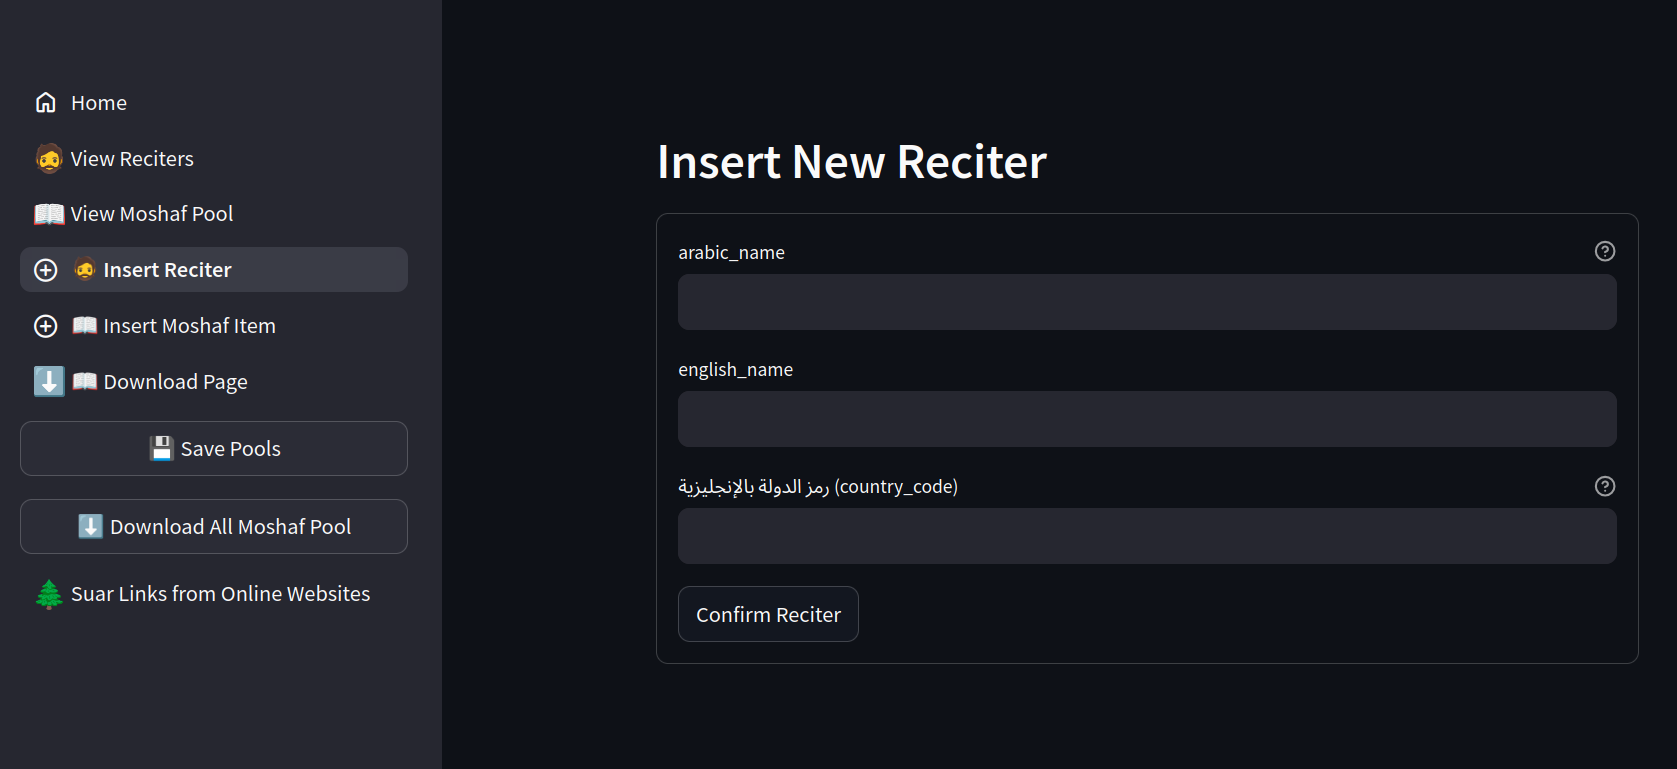
\includegraphics[width=0.8\textwidth]{../figures/ui_insert_new_reciter.png}
\caption{Dialog for inserting a new reciter's details.}
\label{fig:ui_new_reciter}
\end{figure}

\begin{figure}[H]
\centering
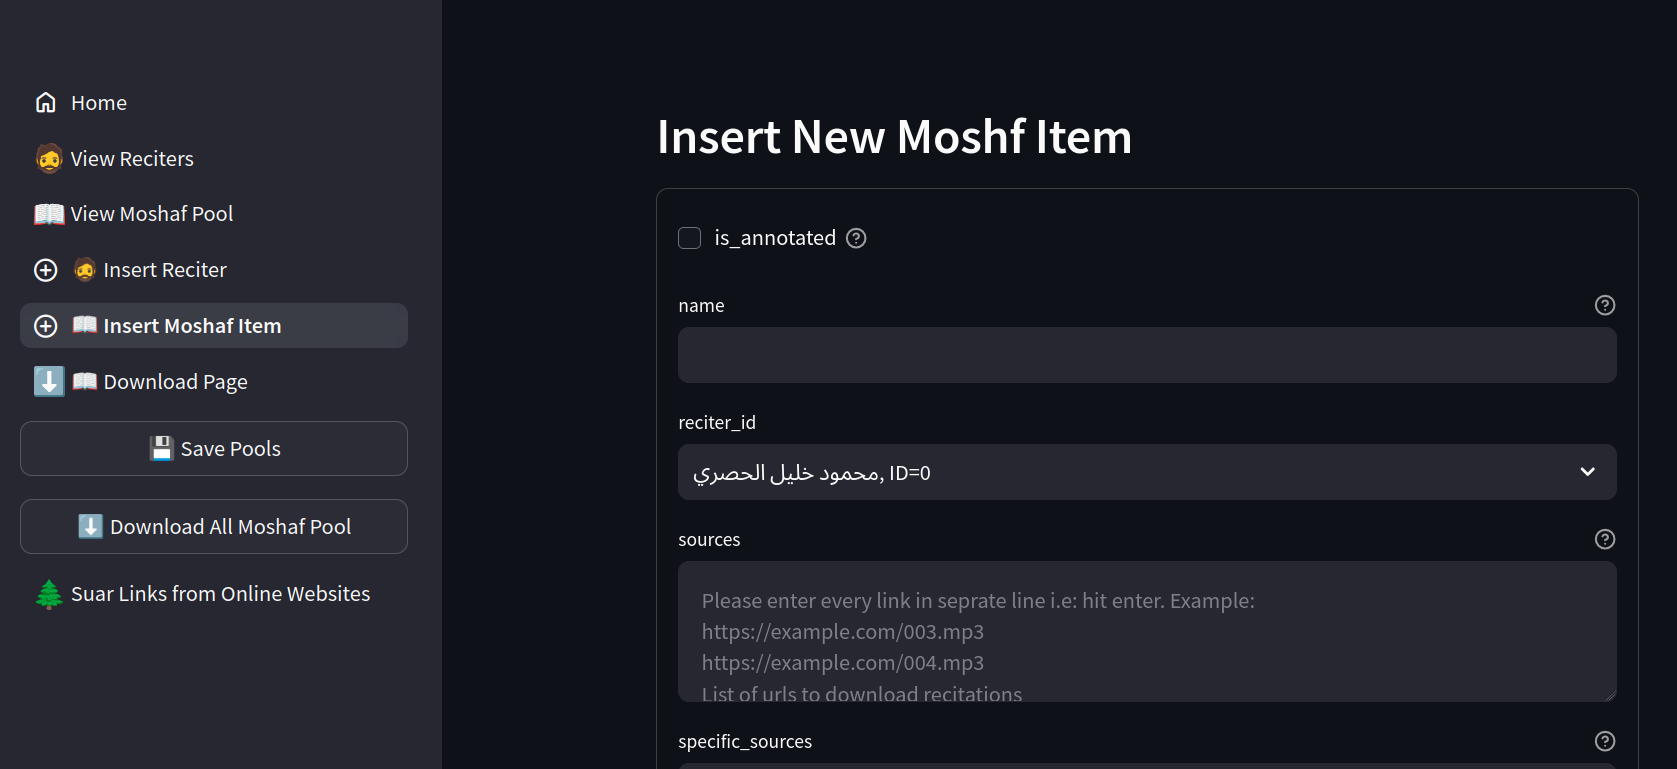
\includegraphics[width=0.8\textwidth]{../figures/ui_inset_new_mohaf.png}
\caption{Dialog for creating and annotating a new Moshaf attribute card.}
\label{fig:ui_new_moshaf}
\end{figure}

\begin{figure}[H]
\centering
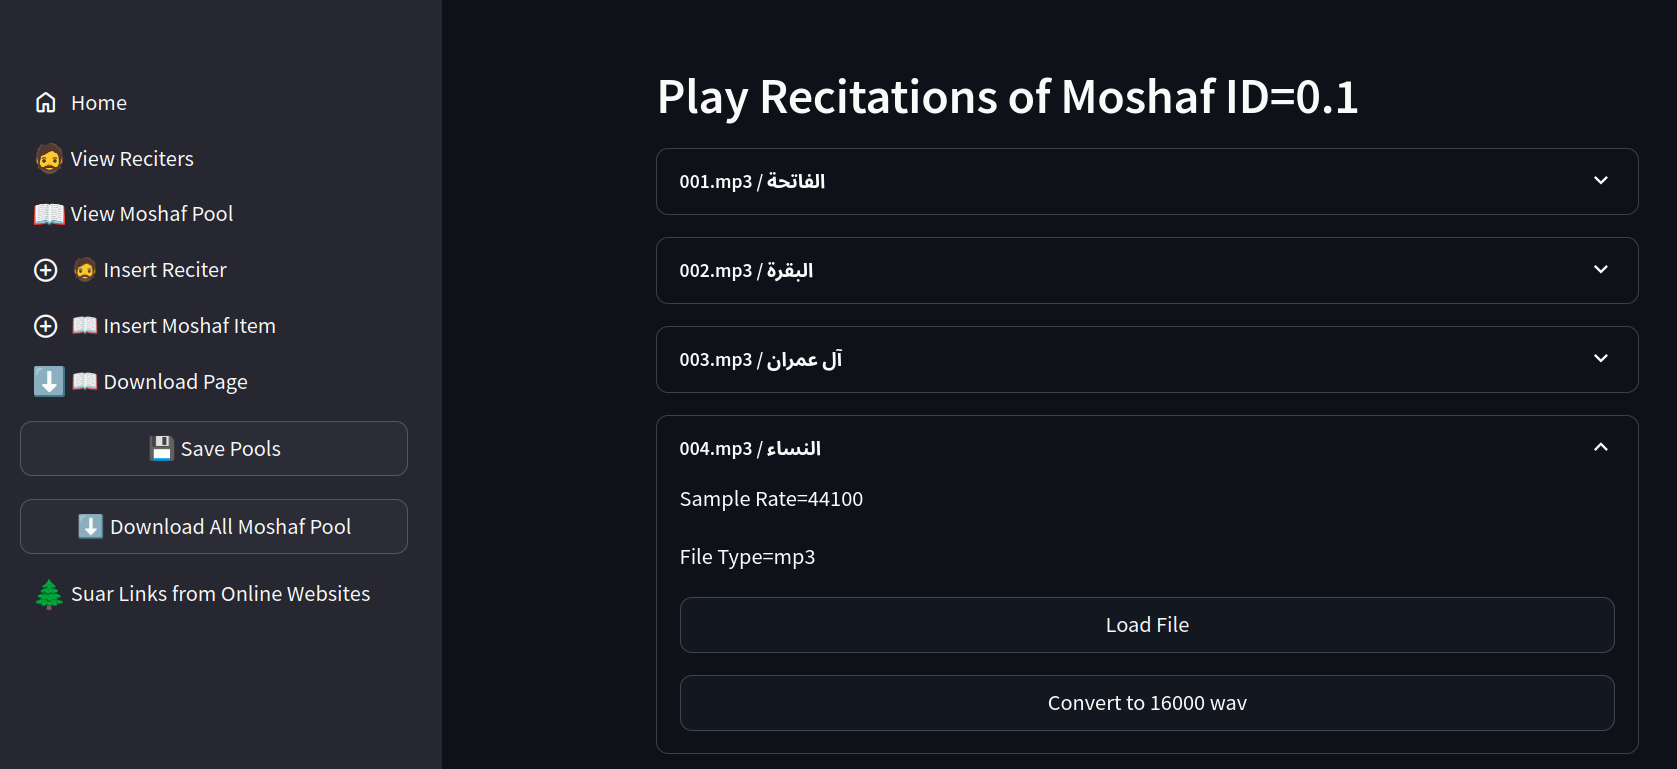
\includegraphics[width=0.8\textwidth]{../figures/ui_play_recitatins.png}
\caption{Interface for viewing a Moshaf's tracks and playing individual recitations.}
\label{fig:ui_play}
\end{figure}






% --------------------------------------------------------



\section{Segmentation of Recitations}

Accurate segmentation is a critical preprocessing step, as Tajweed rules are directly influenced by pause points (\arb{وقف}). To address this, we initially evaluated open-source Voice Activity Detection (VAD) models, including SileroVAD \cite{SileroVAD} and PyAnnotate \cite{Plaquet23}. However, their performance on Quranic recitations was unsatisfactory due to the unique acoustic and prosodic characteristics of Tilawah.

Consequently, we developed a custom segmentation model by fine-tuning the Wav2Vec2-BERT architecture \cite{barrault2023seamless} for frame-level classification, specifically optimized for Quranic audio.

\subsection{Preparation of Segmenter Training Data}

To create a training dataset, we selected \arb{مصاحف} from the EveryAyah\footnote{https://everyayah.com} database that were compatible with SileroVAD v4. This source provided pre-segmented recitations at the verse (ayah) level, which served as our ground truth.

For each Moshaf, we tuned the following segmentation parameters to optimize alignment with the ground truth:
\begin{itemize}
\item \textbf{Threshold:} Detection confidence level.
\item \textbf{Minimum Silence Duration:} Durations below this value trigger segment merging.
\item \textbf{Minimum Speech Duration:} Segments shorter than this value are discarded.
\item \textbf{Padding:} Duration added to the beginning and end of each detected segment.
\end{itemize}

The resulting dataset, comprising eight complete \arb{مصاحف}, is summarized in Table \ref{tab:segmenter_data}.

\begin{longtable}{|p{4cm}|c|c|c|c|c|c|}
\caption{Dataset used for training the custom segmenter, consisting of eight complete Masahif with tuned parameters.}
\label{tab:segmenter_data}\\
\hline
\textbf{Reciter Name (Arabic)} & \textbf{ID} & \textbf{Window Size (Samples)} & \textbf{Threshold} & \textbf{Min Silence (ms)} & \textbf{Min Speech (ms)} & \textbf{Pad (ms)} \\ 
\hline
\endfirsthead
\hline
\arb{محمود خليل الحصري} & 0 & 1536 & 0.3 & 500 & 1000 & 40 \\
\hline
\arb{محمد صديق المنشاوي} & 1 & 1536 & 0.3 & 400 & 1000 & 20 \\
\hline
\arb{عبد الباسط عبد الصمد} & 2 & 1536 & 0.3 & 400 & 700 & 20 \\
\hline
\arb{محمود علي البنا} & 3 & 1536 & 0.3 & 400 & 700 & 20 \\
\hline
\arb{على الحذيفي} & 5 & 1536 & 0.3 & 350 & 700 & 5 \\
\hline
\arb{أيمن رشدي سويد} & 6 & 1536 & 0.3 & 500 & 1000 & 10 \\
\hline
\arb{محمد أيوب} & 7 & 1536 & 0.3 & 400 & 1000 & 10 \\
\hline
\arb{إبراهيم الأخضر} & 8 & 1536 & 0.3 & 390 & 700 & 30 \\
\hline
\end{longtable}

\subsubsection{Data Augmentation}

To improve model robustness and generalize across various recording conditions, we employed data augmentation using the Audiomentations library. The augmentation strategy replicated SileroVAD's noise profile and was applied to 40\% of the samples. With additional:
\begin{itemize}
\item \texttt{TimeStretch} (0.8x-1.5x) to simulate recitation speeds
\item Sliding window truncation (1-second windows) for long samples instead of exclusion
\end{itemize}

\subsection{Segmenter Training}

The Wav2Vec2BERT model was fine-tuned for frame-level classification over a single epoch. The architecture of our VAD model compared to standard streaming models is illustrated in the figure below.

\begin{figure}[H]
\centering
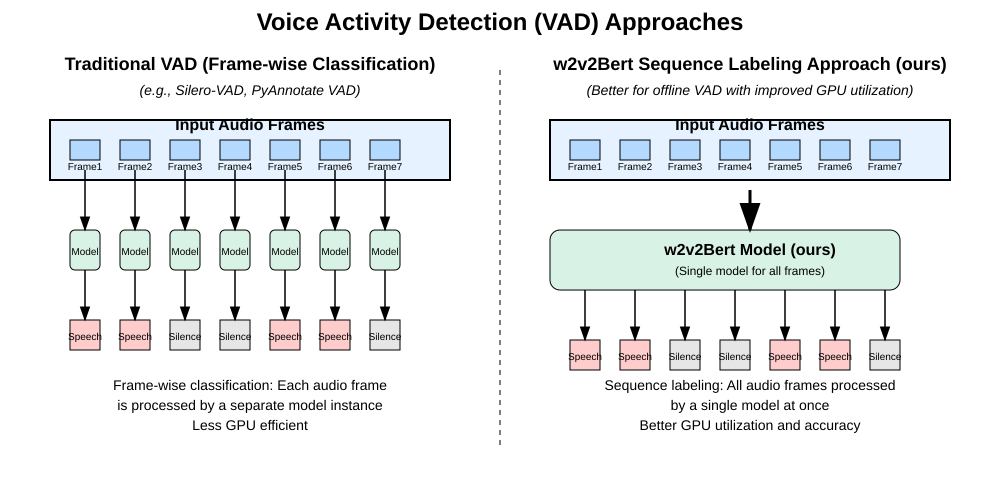
\includegraphics[width=0.8\textwidth]{../figures/vad-arch.png}
\caption{Architecture of the fine-tuned Wav2Vec2-BERT model for frame classification, compared to a standard streaming model.}
\label{fig:vad_arch}
\end{figure}

The model's performance on unseen \arb{مصاحف} demonstrated high accuracy, as shown in Table \ref{tab:vad_results}.

\begin{longtable}{|l|c|}
\caption{Evaluation results of the segmentation model on a held-out test set of Masahif, showing superior performance. The quality of the segmenter was validated by processing our entire dataset, where it maintained this high level of performance. The only exceptions were edge cases involving extremely fast recitation (\arb{حدر}), which is an expected limitation.}
\label{tab:vad_results}\\
\hline
\textbf{Metric} & \textbf{Value} \\ 
\hline
\endfirsthead
\hline
Test Loss & 0.0277 \\
\hline
Test Accuracy & 0.9935 \\
\hline
Test F1 Score & 0.99476 \\
\hline
\end{longtable}






% --------------------------------------------------------------------

\section{Transcribe Segmented Parts}

We employed Tarteel ASR \cite{tarteel_whisper_ar_quran} (Whisper fine-tuned on Quranic recitations \cite{radford2023robust}). To handle its 30-second limit, we used sliding window truncation (10-second windows), with verification in the next step. We used vlLM library because it is really fast thanks to Employing Paged Attention \cite{kwon2023efficient}.





% ------------------------------------------------------------------------





\section{Verification of Segmentation and Transcription}
\section{Data Verification}

To ensure the highest quality of our dataset, we developed a custom verification interface using Streamlit\footnote{https://streamlit.io/}. We manually inspect 50-75 randomly selected samples per Moshaf, focusing on the following aspects:

\begin{itemize}
\item \textbf{Segmentation Quality:} Assessing the accuracy of pause detection to determine if adjustments were needed, including:
\begin{itemize}
    \item Increasing or decreasing padding durations
    \item Merging adjacent segments
    \item Splitting undetected segments
\end{itemize}
\item \textbf{Qalqala (\arb{القلقلة}) Duration Inspection:} Verifying that segments containing Qalqala (\arb{قلقة}) are fully captured without being truncated by brief silences, ensuring the acoustic feature remains intact.
\item \textbf{Hams (\arb{همس}) Duration Inspection:} Similarly checking segments for Hams (a whispered or airy phonation) to ensure the subtle release of air was not missed by the segmenter.
\end{itemize}

\begin{figure}[H]
\centering
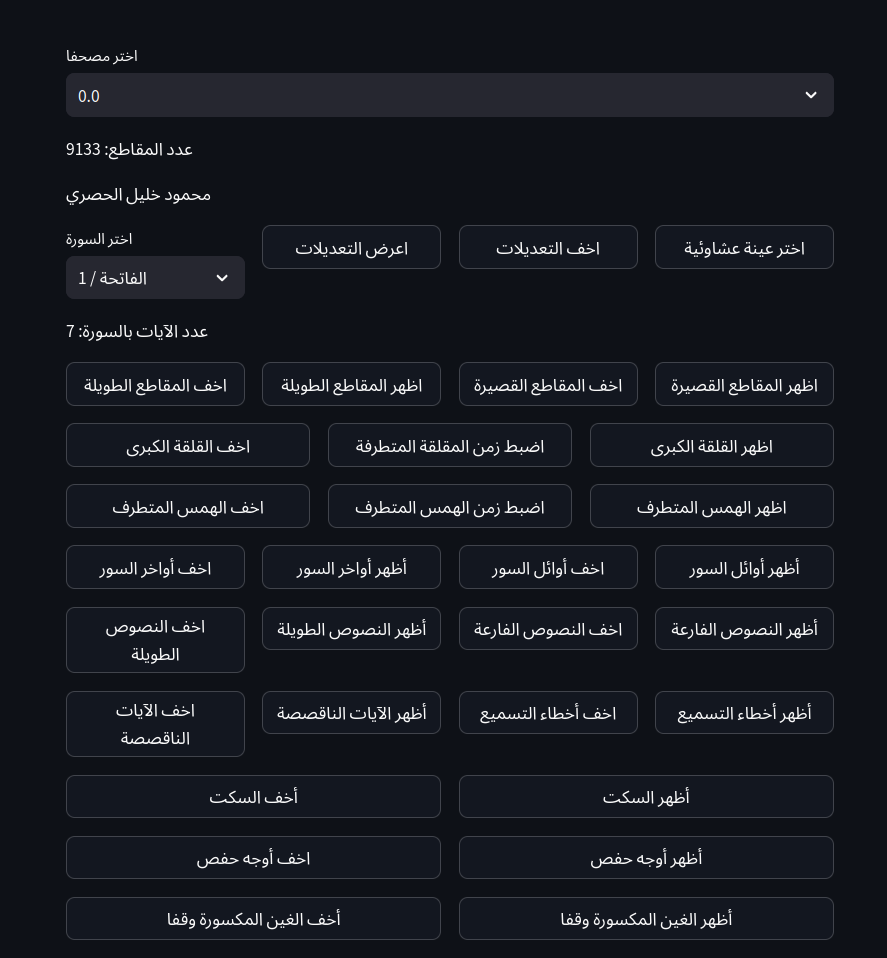
\includegraphics[width=0.8\textwidth]{../figures/data_verfication_ui.png}
\caption{The Streamlit-based UI for manually verifying segmentation quality and phonetic feature integrity.}
\label{fig:verification_ui}
\end{figure}

\begin{figure}[H]
\centering
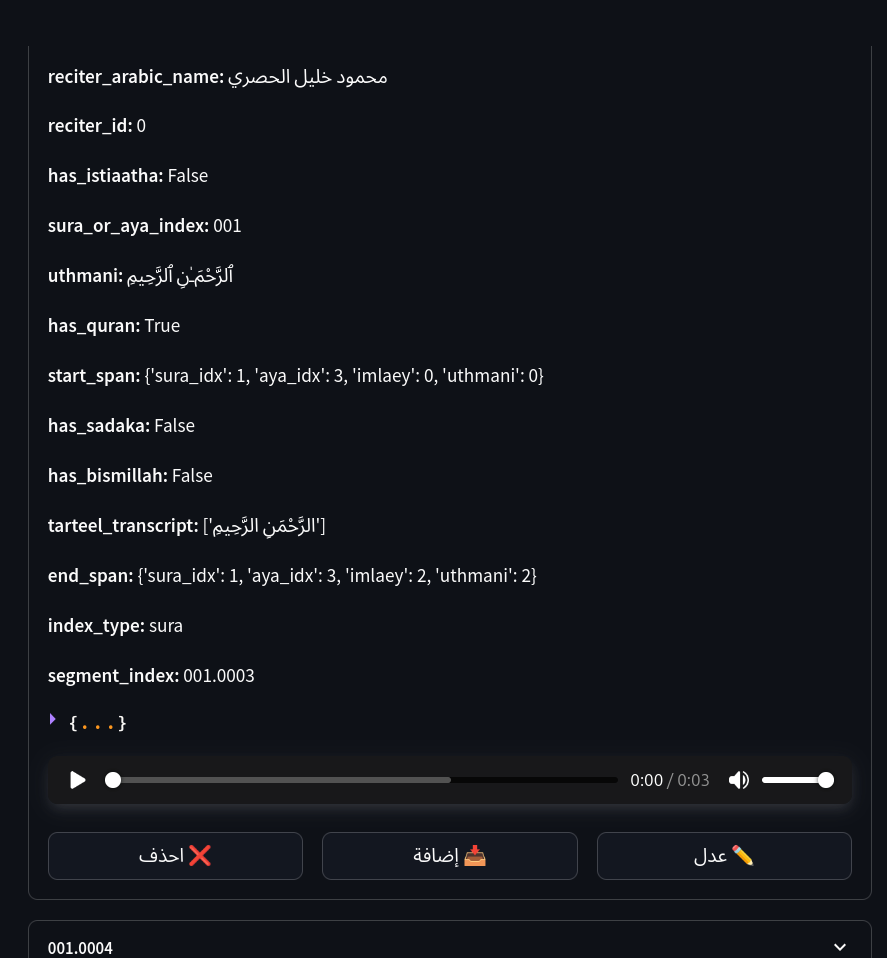
\includegraphics[width=0.8\textwidth]{../figures/data_annotation_ui_editing.png}
\caption{The editing view within the verification UI, allowing for manual correction of segment boundaries.}
\label{fig:annotation_ui}
\end{figure}

After completing the annotation process for a Moshaf, the defined correction operations were programmatically applied to the entire dataset to ensure consistency.

\textbf{Note:} Moshaf 25.0 was excluded from the final dataset due to irreconcilably poor segmentation quality.

\subsection{Transcription Verification: A \arb{تسميع}-Inspired Algorithm}

To validate the accuracy of the automated speech recognition (ASR) output, we developed a verification algorithm inspired by Tasmeea (\arb{تسميع})—the traditional practice where a student recites for a teacher to correct mistakes. This statistical algorithm operates under the core assumption that the input recitations are 100\% correct, and any errors originate from the ASR model (Tarteel model).

The algorithm proceeds through the following steps:
\begin{enumerate}
\item \textbf{Automatic Matching:} Segments are automatically matched to the canonical Quranic text.
\item \textbf{Discrepancy Identification:} The system identifies missing verses, words, or unexpected additions in the transcription.
\item \textbf{Manual Correction:} flagged discrepancies are presented for manual review and correction within our annotation UI, completing the \arb{تسميع} feedback loop.
\end{enumerate}
















\begin{algorithm}[H]
\caption{Tasmeea Algorithm}
\label{alg:tasmeea}
\begin{algorithmic}[1]
\REQUIRE $text\_segments = [s_1, s_2, \dots, s_n]$, $sura\_idx$, 
          $overlap\_words = 6$, $window\_words = 30$, 
          $acceptance\_ratio = 0.5$, flags for special phrases
\ENSURE List of tuples $(match, ratio)$ per segment

\STATE $aya \leftarrow 1$ \COMMENT{Start at first verse}
\STATE $penalty \leftarrow 0$
\FOR{each segment $s_i$ in $text\_segments$}
    \STATE $norm\_text \leftarrow$ normalize($s_i$) \COMMENT{Remove spaces/diacritics}
    \STATE $min\_win \leftarrow window\_words - 10$, $max\_win \leftarrow window\_words + 10$
    \STATE $start\_range \leftarrow [-(overlap + penalty), (overlap + \max(window\_words, max\_win) + penalty]$
    
    \IF{first segment \AND $include\_istiaatha$}
        \STATE Check istiaatha special case
    \ELSIF{last segment \AND $include\_sadaka$}
        \STATE Check sadaka special case
    \ENDIF
    
    \STATE $best\_ratio \leftarrow 0$, $best\_match \leftarrow \text{null}$
    \FOR{each start position $p$ in $start\_range$}
        \FOR{each window size $w \in [min\_win, max\_win]$}
            \STATE $c \leftarrow$ extract candidate at ($aya$, $p$, $w$)
            \STATE $dist \leftarrow \text{edit\_distance}(norm\_text, c)$
            \STATE $ratio \leftarrow 1 - \min(dist, |norm\_text|) / |norm\_text|$
            \IF{$ratio > best\_ratio$ \OR ($ratio = best\_ratio$ \AND $|p| < |best\_start|$)}
                \STATE update $best\_ratio$, $best\_match$, $best\_start$, $best\_window$
            \ENDIF
        \ENDFOR
    \ENDFOR
    
    \IF{$best\_ratio < acceptance\_ratio$}
        \STATE output (null, $best\_ratio$)
        \STATE $penalty \leftarrow max\_win$
        \STATE $aya \leftarrow aya + 1$ \COMMENT{Default advance}
    \ELSE
        \STATE output ($best\_match$, $best\_ratio$)
        \STATE $aya \leftarrow aya + best\_start + best\_window$
        \STATE $penalty \leftarrow 0$
    \ENDIF
\ENDFOR
\STATE \textbf{Complexity:} $O(N \cdot W \cdot L^2)$ \COMMENT{$N$=segments, $W$=window size, $L$=segment length}
\end{algorithmic}
\end{algorithm}
